\subsection{Simulaciones}

Ya con el valor de los componentes se utilizo LTSPICE para simular las etapas por separado y compararlas con la herramienta LAPLACE.
Finalmente se pusieron en cascada las etapas y se ajusto la ganancia para cumplir con los requerimientos.

\subsubsection{Realimentacion positiva (Sallen-Key)}

Para la primer etapa se armo el filtro con los componentes calculados y se configuro la herramienta LAPLACE con los parametros de la primer FT.

\begin{figure}[H]
    \centering
    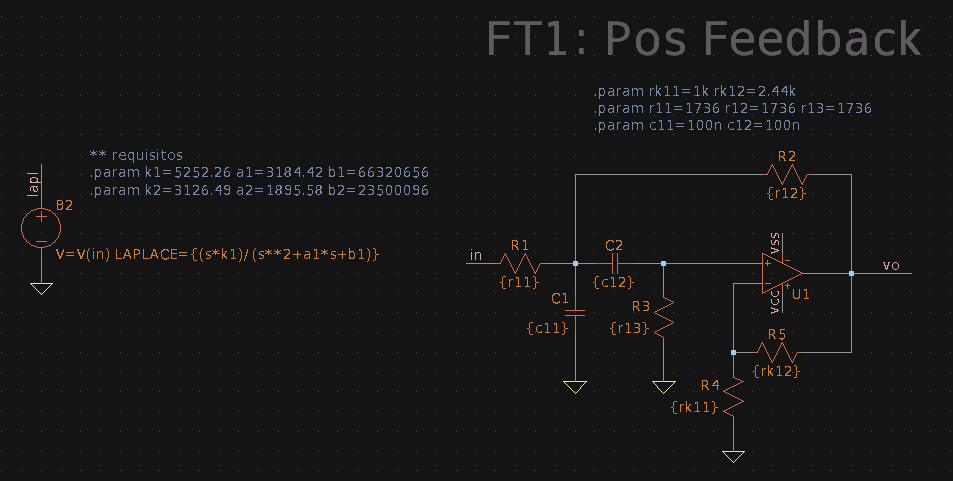
\includegraphics[scale=.4]{Secciones/Circ1/img/schLpPos.png}
    \caption{Circuito para primer etapa.}
    \label{schPos}
\end{figure}

\noindent $>>$ \texttt{Comparando ambas respuestas:}

\begin{figure}[H]
    \centering
    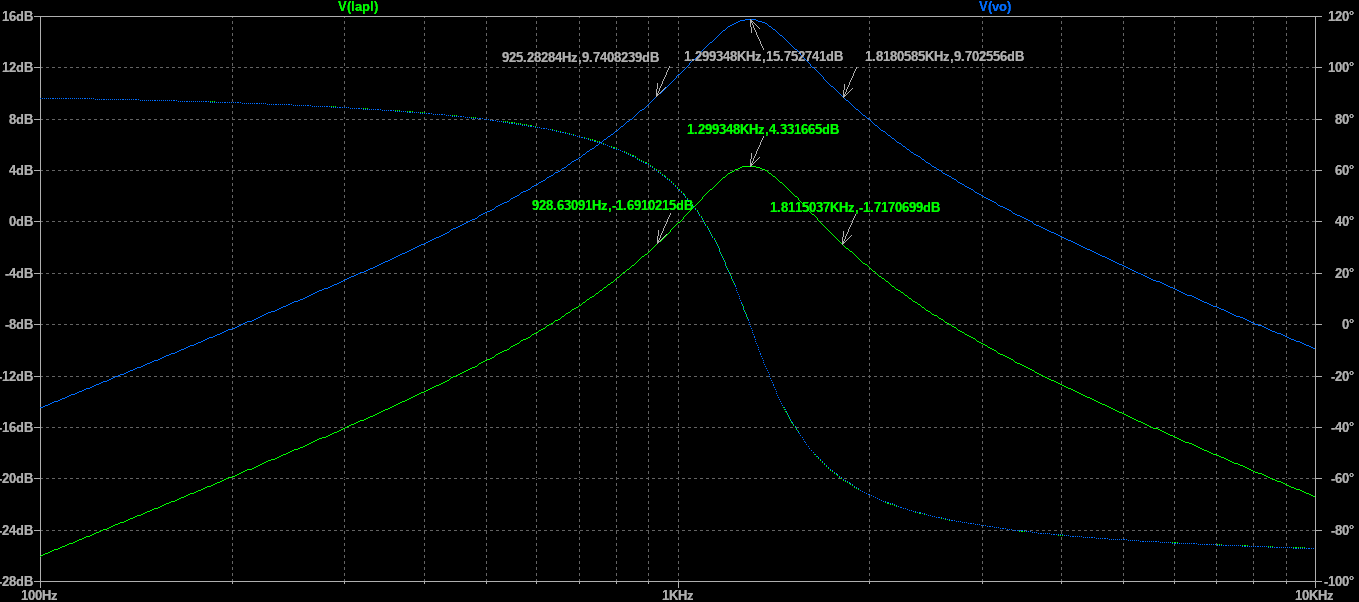
\includegraphics[scale=.3]{Secciones/Circ1/img/lpVsPos.png}
    \caption{Laplace vs primer etapa.}
    \label{schPos}
\end{figure}

Ignorando la diferencia de magnitud entre ambas respuestas se tiene para la primer etapa un pasa-banda con frecuencia central de 1.3KHz aprox. y ancho de banda de 893Hz, que es casi identica a la respuesta de LAPLACE con frecuencia central 1.3KHz y ancho de banda 883Hz.

\subsubsection{Realimentacion negativa}

Para la segunda etapa se armo el filtro con los componentes calculados y se configuro la herramienta LAPLACE con los parametros de la segunda FT.

\begin{figure}[H]
    \centering
    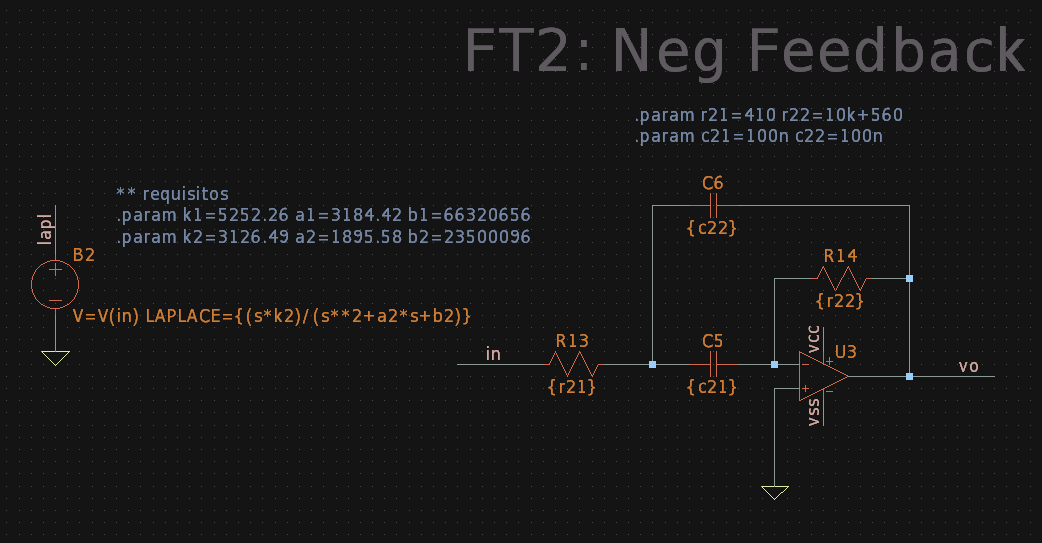
\includegraphics[scale=.4]{Secciones/Circ1/img/schLpNeg.png}
    \caption{Circuito para segunda etapa.}
    \label{schPos}
\end{figure}

\begin{figure}[H]
    \centering
    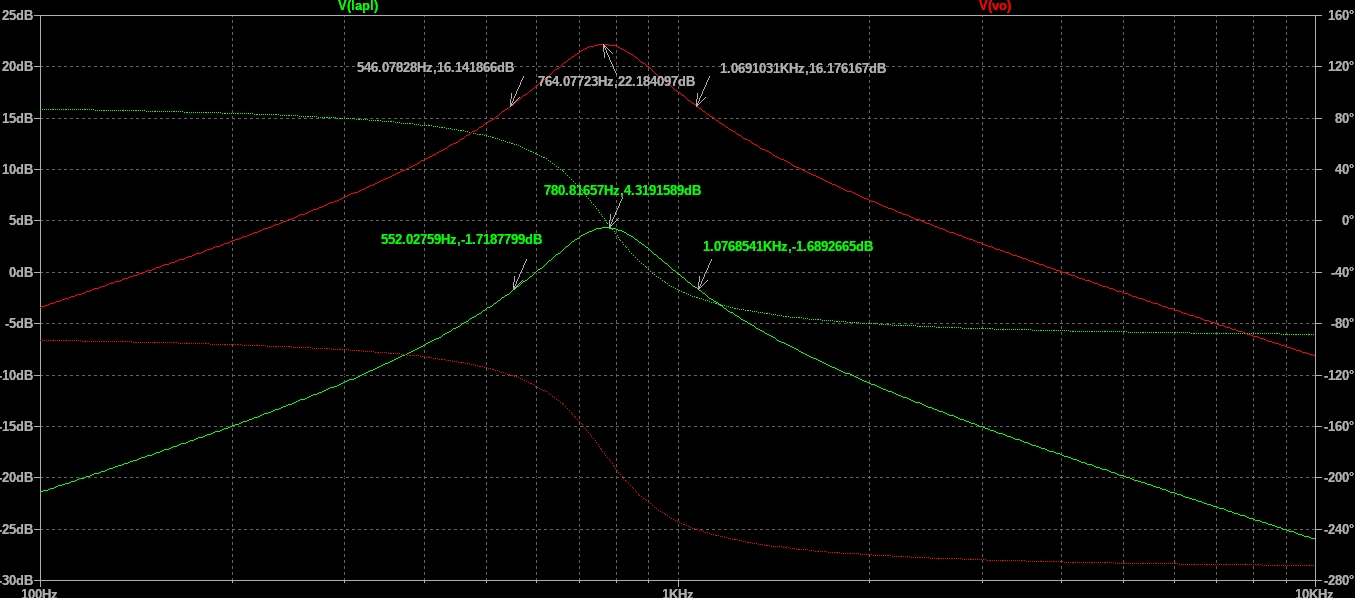
\includegraphics[scale=.3]{Secciones/Circ1/img/lpVsNeg.png}
    \caption{Laplace vs segunda etapa.}
    \label{schPos}
\end{figure}

Ignorando la diferencia de magnitud entre ambas respuestas se tiene para la segunda etapa un pasa-banda con frecuencia central de 764Hz aprox. y ancho de banda de 454Hz, en este caso algo diferente a la respuesta de LAPLACE con frecuencia central 780Hz y ancho de banda 448Hz. En efecto aqui se observo como al alejarse del valor calculado para las resistencias, en pos de hacer sencilla la implementacion circuital, tambien nos alejamos de la FT teorica.

\subsubsection{Filtro final}

Luego se unieron las etapas y se configuro LAPLACE con la funcion de transferencia final.

\begin{figure}[H]
    \centering
    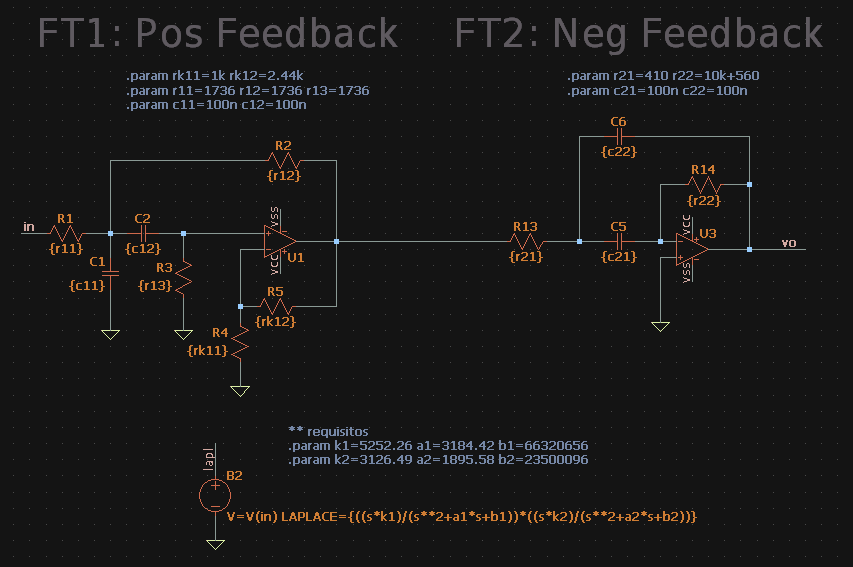
\includegraphics[scale=.4]{Secciones/Circ1/img/schLpBP.png}
    \caption{Filtro multi-etapa.}
    \label{schPos}
\end{figure}

Comparando las respuestas se notaron las diferencias en magnitud y fase respecto de la respuesta ideal.

\begin{figure}[H]
    \centering
    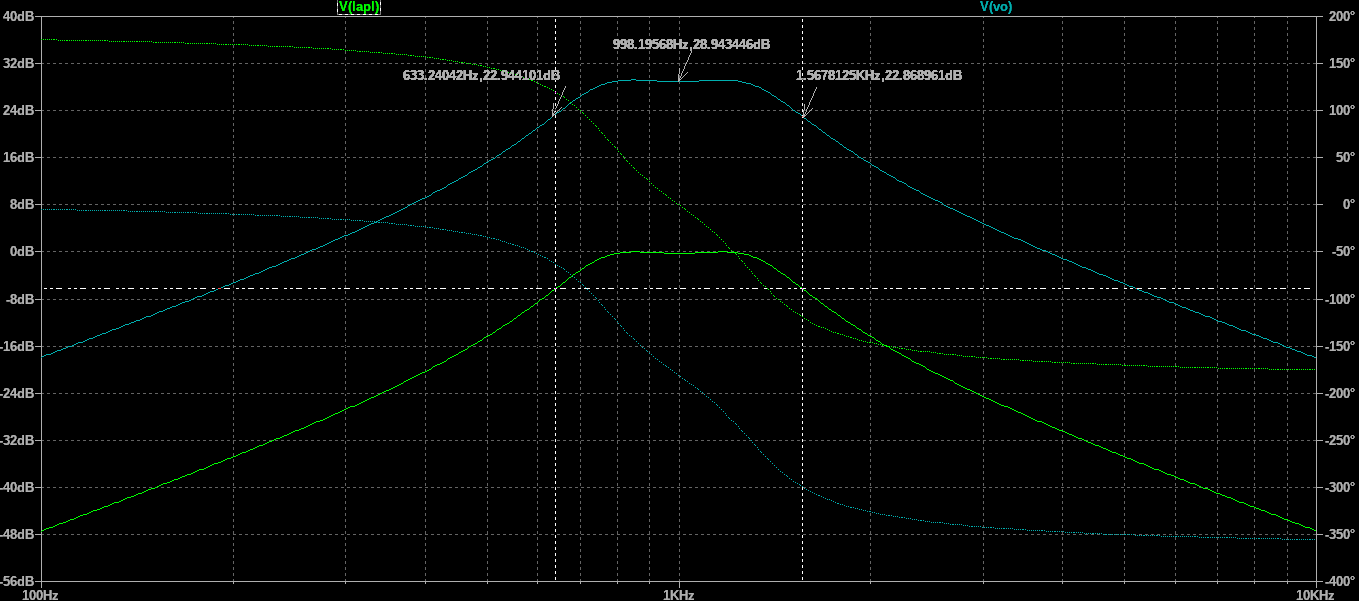
\includegraphics[scale=.3]{Secciones/Circ1/img/lpVsBP.png}
    \caption{Laplace vs filtro multi-etapa.}
    \label{schPos}
\end{figure}

Para terminar los ajustes de ganancia y fase se agrego una etapa inversora con una atenuacion de 28.9dB.

\begin{align*}
    att &= 28.9dB \longrightarrow att = 10^{\frac{28.9}{20}} = 27.86 = \frac{1}{k} \longrightarrow k \cong 0.035 \\
    k &= - \frac{R2}{R1} \longrightarrow \textbf{R1=100k$\Omega$ y R2=3.3k$\Omega$+220$\Omega$}
\end{align*} \\

\noindent $>>$ \texttt{Obteniendo el circuito final:}

\begin{figure}[H]
    \centering
    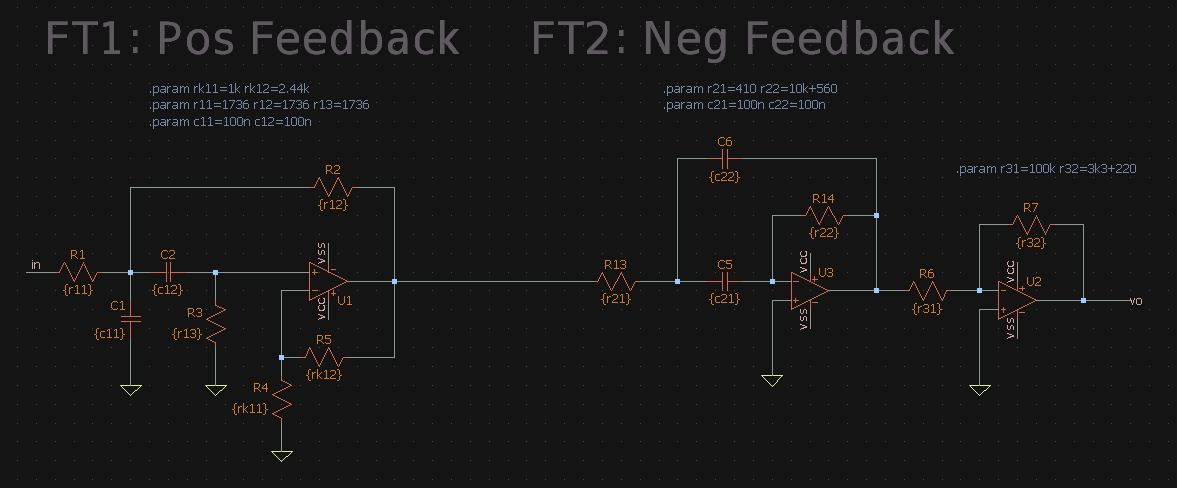
\includegraphics[scale=.35]{Secciones/Circ1/img/schBPFinal.png}
    \caption{Circuito final.}
    \label{schPos}
\end{figure}

Y comparando con los requisitos tenemos respuestas muy similares.

\begin{figure}[H]
    \centering
    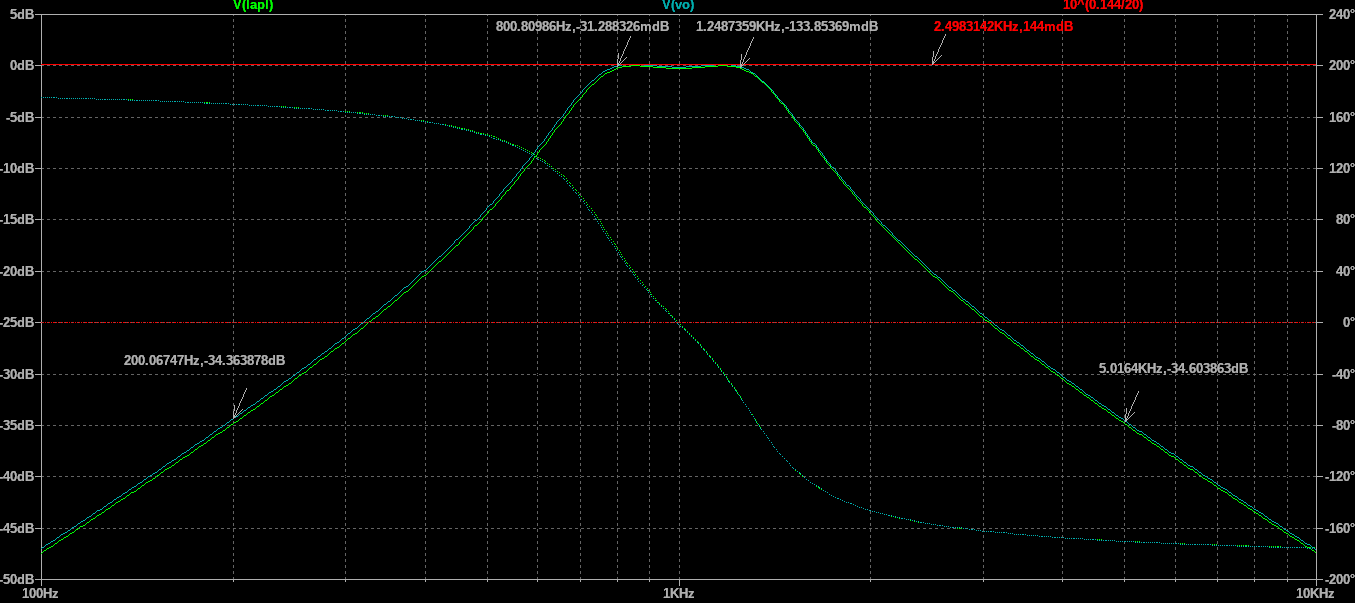
\includegraphics[scale=.3]{Secciones/Circ1/img/lpVsBPFinal.png}
    \caption{Laplace vs circuito final.}
    \label{schPos}
\end{figure}

Con lo que se tiene una atenuacion maxima entre los 800 y 1250Hz de 0.27dB (algo superior a la requerida) y una atenuacion mayor a 34dB para los 200Hz y 5KHz respectivamente. Por lo que se sintetizo un filtro casi identico al requerido.